% BUSINESS CARD template
% created by Karol Kozioł (www.karol-koziol.net)
% for ShareLaTeX - online LaTeX editor (www.sharelatex.com)
% May 2013
% Addition: QR code support
% by Dieter Castel
% February 2015

\documentclass[10pt]{article}
\usepackage[dvips]{graphicx}
\usepackage[utf8]{inputenc}
\usepackage[T1]{fontenc}
\usepackage{xcolor}
\usepackage{tikz}
%Add package to provide QR code
\usepackage{qrcode}

\usepackage{geometry}
\geometry{total={210mm,297mm},hmargin=10mm,vmargin=2mm}

\pagestyle{empty}

\renewcommand\familydefault{\sfdefault}
\usepackage{tgadventor}

%%% BUSINESS CARD SIZE
\newlength{\cardw}
\newlength{\cardh}
%% ISO 7810 size: 85.60mm × 53.98mm
\setlength{\cardw}{85.60mm}
\setlength{\cardh}{53.98mm}
%% European size: 85mm × 55mm
% \setlength{\cardw}{85mm}
% \setlength{\cardh}{55mm}
%% US size: 3.5 in × 2 in
%\setlength{\cardw}{3.5in}
%\setlength{\cardh}{2in}


%%% DEFINE USER DATA
\newcommand{\Surname}{
Doe
}%
\newcommand{\Firstname}{
Joe
}%
\newcommand{\Name}{
{\textbf{\Firstname \Surname}} 
}% No size here so it's easier to try out multiple sizes
\newcommand{\Description}{
{CEO of XYZ Company}
}% No size here so it's easier to try out multiple sizes
\newcommand{\Email}{
joe.doe@emails.com
}%
\newcommand{\Phone}{
+44 123456789
}%
\newcommand{\Website}{
http://joedoe.net
}%
\newcommand{\Twitter}{
@JoeDoeTweets
}%

%MeCard command to include in QR Code
\newcommand{\MeCard}{
MECARD:N:\Firstname,\Surname;TEL:\Phone;EMAIL:\Email;URL:\Website;;
}
%Content of the QR Code
\newcommand{\TheQRContent}{
\MeCard
}

%Make actual QR code
\newcommand{\MyQRC}{
\qrcode[nolinks, height=0.3\cardw]{\TheQRContent}
}

\begin{document}
% Example with QR code 
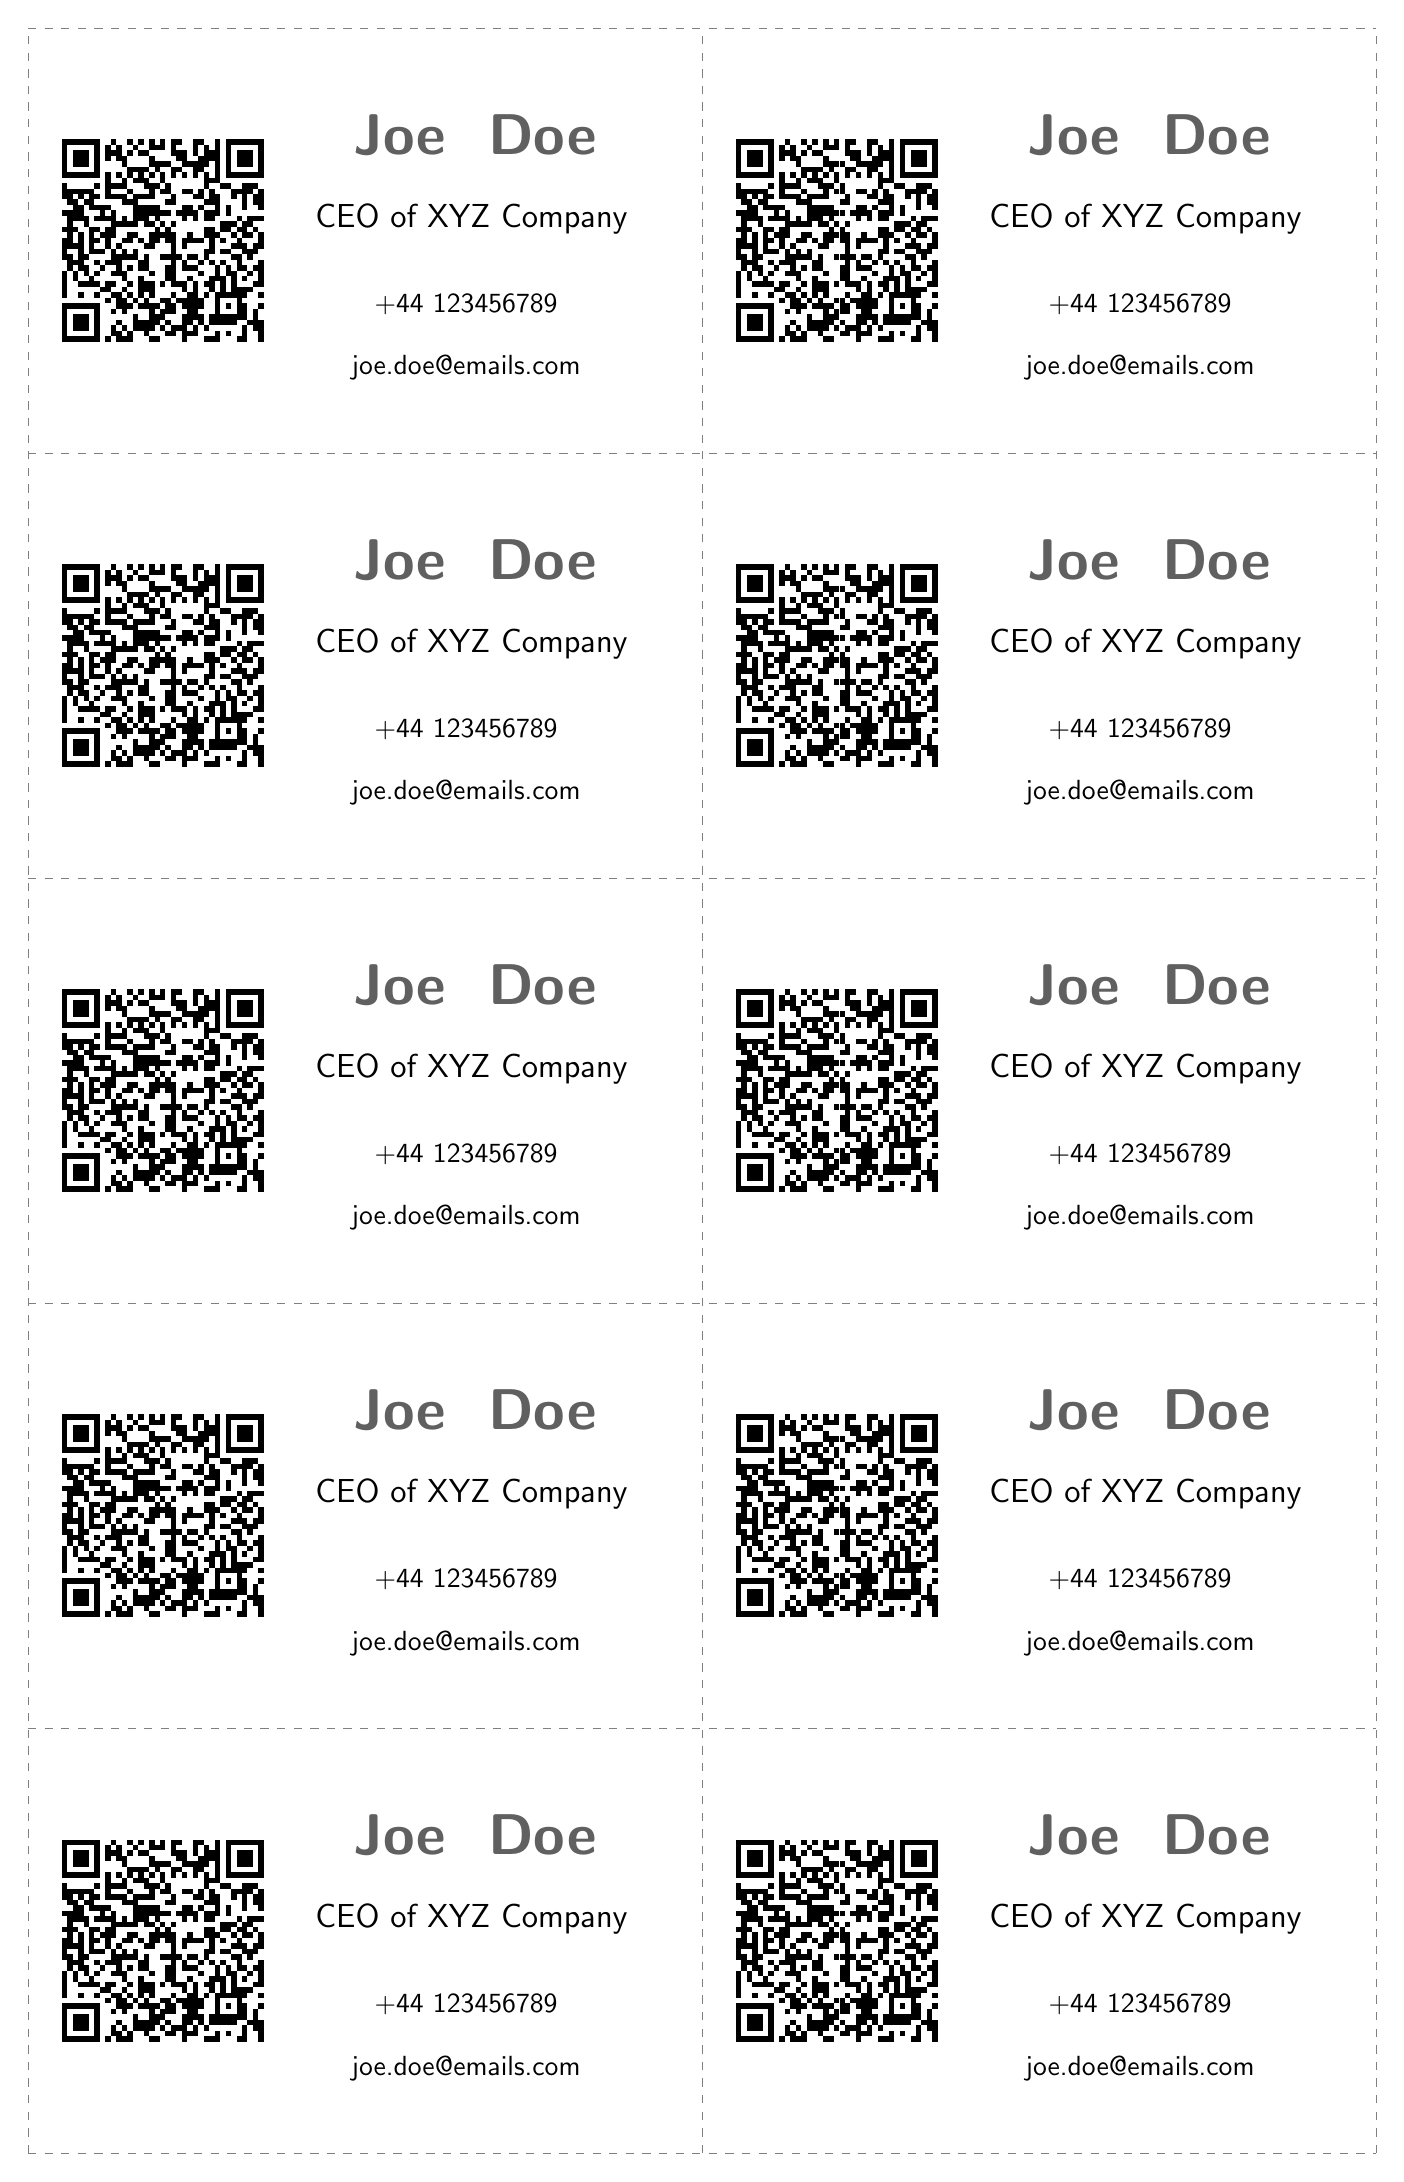
\begin{tikzpicture}
% grid
\foreach \i in {0,1,2,3,4,5} \draw[very thin, gray,dashed] (0,\i*\cardh) -- (2*\cardw,\i*\cardh);
\foreach \j in {0,1,2} \draw[very thin, gray,dashed] (\j*\cardw,0) -- (\j*\cardw,5*\cardh);
% card content
\foreach \i in {0,1} \foreach \j in {0,1,2,3,4} {
   % Add QR Code to the card 
   \node at (\i*\cardw+0.2\cardw,\j*\cardh+0.5\cardh){\MyQRC};
% center text
   \node[black!25!gray] at (\i*\cardw+0.65\cardw,\j*\cardh+0.75\cardh) {\huge \Name};
   \node at (\i*\cardw+0.65\cardw,\j*\cardh+0.55\cardh) {\large \Description};
   \node at (\i*\cardw+0.65\cardw,\j*\cardh+0.35\cardh) {\Phone};
   \node at (\i*\cardw+0.65\cardw,\j*\cardh+0.2\cardh) {\Email};
};
\end{tikzpicture}

\newpage
% Original ShareLaTeX example with logo
\begin{tikzpicture}
% grid
\foreach \i in {0,1,2,3,4,5} \draw[very thin, gray,dashed] (0,\i*\cardh) -- (2*\cardw,\i*\cardh);
\foreach \j in {0,1,2} \draw[very thin, gray,dashed] (\j*\cardw,0) -- (\j*\cardw,5*\cardh);
% card content
\foreach \i in {0,1} \foreach \j in {0,1,2,3,4} {
   % Add logo to the card 
   \node at (\i*\cardw+0.2\cardw,\j*\cardh+0.5\cardh) {\includegraphics[width=0.2\cardw]{logo}};
% center text
   \node[black!25!gray] at (\i*\cardw+0.65\cardw,\j*\cardh+0.75\cardh) {\huge \Name};
   \node at (\i*\cardw+0.65\cardw,\j*\cardh+0.55\cardh) {\large \Description};
   \node at (\i*\cardw+0.65\cardw,\j*\cardh+0.35\cardh) {\Phone};
   \node at (\i*\cardw+0.65\cardw,\j*\cardh+0.2\cardh) {\Email};
% align text left %    \node[black!25!gray,right] at (\i*\cardw+0.4\cardw,\j*\cardh+0.75\cardh) {\huge \Name};
%    \node[right] at (\i*\cardw+0.4\cardw,\j*\cardh+0.55\cardh) {\large \Description};
%    \node[right] at (\i*\cardw+0.4\cardw,\j*\cardh+0.35\cardh) {\Phone};
%    \node[right] at (\i*\cardw+0.4\cardw,\j*\cardh+0.2\cardh) {\Email};
};

\end{tikzpicture}

\newpage
% Other example with centred (custom size) Name, QR Code and twitter. 
\begin{tikzpicture}
% grid
\foreach \i in {0,1,2,3,4,5} \draw[very thin, gray,dashed] (0,\i*\cardh) -- (2*\cardw,\i*\cardh);
\foreach \j in {0,1,2} \draw[very thin, gray,dashed] (\j*\cardw,0) -- (\j*\cardw,5*\cardh);
% card content
\foreach \i in {0,1} \foreach \j in {0,1,2,3,4} {
   % Add QR code to the card 
   \node at (\i*\cardw+0.23\cardw,\j*\cardh+0.35\cardh){\MyQRC};
% center text for Name and Description
   \node at (\i*\cardw+0.50\cardw,\j*\cardh+0.83\cardh) {\fontsize{26pt} \selectfont \Name};
   \node at (\i*\cardw+0.50\cardw,\j*\cardh+0.67\cardh) {\fontsize{20pt} \selectfont \Description};
% Aligin text left for other info
   \node[right] at (\i*\cardw+0.43\cardw,\j*\cardh+0.50\cardh) {\Email};
   \node[right] at (\i*\cardw+0.43\cardw,\j*\cardh+0.40\cardh) {\Website};
   \node[right] at (\i*\cardw+0.43\cardw,\j*\cardh+0.30\cardh) {\Phone};
   \node[right] at (\i*\cardw+0.43\cardw,\j*\cardh+0.20\cardh) {\Twitter};
};
\end{tikzpicture}
\end{document}
